\section{Neuronales Netz}\label{sec:nn}
In der Analyse der Daten (siehe\autoref{sec:analyse}) wurde die Korrelation 
der verschiedenen Eigenschaften von Wohnungen untersucht. Die dort gefundenen
Zusammenhänge können nun verwendet werden, um die Eingaben für das Neuronale 
Netz anzupassen. Dies ist notwendig, da ein neuronales Netz effizienter
die gewünschte Funktion erlernen kann, wenn die Eingaben aussagekräftige 
Informationen darstellen. \\
Aus diesem Grund werden für das Netz nicht einfach die in der Aufgabenstellung 
gegebenen Attribute verwendet sondern Attribute die eine hohe Korrelation besitzen
zusammengefasst und Attribute die einen geringen Einfluss auf die Bewertung haben
nicht verwendet. \\
Die Folgende Auflistung zeigt die Attribute, die verwendet werden: 
\begin{itemize}
    \item \textbf{Kosten pro Quadratmeter:} Miete, Quadratmeter
    \item \textbf{Gesamtkosten:} Nebenkosten, Miete, Kaution
    \item \textbf{Kinderfreundlichkeit:} Schule, Kindergarten
    \item \textbf{Mobilität:} Entfernung
    \item \textbf{Ausstattung:} Möbliert
    \item \textbf{Zimmerzahl}
\end{itemize}

Ausgeschlossene Attribute mit Korrelationswerten unter 0,1 beziehungsweise -0,1 sind:\\
Stockwerk, Heizung, Hausmeister, S-Bahn, Alter, Aufzug, Lage, Küche, Bad, Balkon, Terrasse, Kehrwoche, 
und Garage.

\paragraph{Kosten pro Quadratmeter}
Dieses Attribut löst die Korrelation zwischen Miete und der Anzahl der Quadratmeter und kann 
stellt so eine aussagekräftigere Eigenschaft für die Bewertung des Preis-Leistungsverhältnisses dar.


\subsection{Umwandlung der Daten in numerische Werte}
Im nächsten Schritt müssen alle Werte in numerische Werte umgewandelt werden. 
\begin{itemize}
    \item \textit{num-num}: Bei diesen Werten wird ganz einfach der Mittelwert gebildet. 
    \item \textit{über/unter}: Die Randwerte werden als normale Werte angesehen. 
    \item \textit{nah/erreichbar/fern}: Hier bietet es sich an das Attribut als \textit{Entfernung zu ...} umzuschreiben. 
                So kann für \textit{nah} der Minimalwert und für \textit{fern} der Maximalwert verwendet werden.
    \begin{itemize}
        \item nah: 0
        \item erreichbar: 0,5
        \item fern: 1
    \end{itemize}
    \item \textit{Boolean}: Für Werte die entweder erfüllt oder nicht erfüllt sind, wird 0 (nicht erfüllt) und 1 (erfüllt) verwendet.
\end{itemize}

Berechnungen die durchgeführt werden müssen: 
\begin{equation}
        MieteProQuadratmeter = \frac{Miete}{Quadratmeter}
\end{equation}
\begin{equation}
    Gesamtkosten = Miete + Nebenkosten + Kaution
\end{equation}
\begin{equation}
    Kinderfreundlichkeit = \frac{Schule + Kindergarten}{2}
\end{equation}

\subsection{Normierung der Daten}
Um eine Normierung der Daten durchzuführen müssen zunächst die Maximalwerte der 
jeweiligen Attribute definiert werden. Die Werte werden anschließend auf Werte 
zwischen 0 und 1 normiert. Dies ist notwendig, da eine Vorgewichtung der Attribute
vermieden werden soll.

\subsection{Initiale Gewichtung der Neuronen}
Die initialen Gewichte für das Netz werden zufällig gesetzt. Diese werden in der Lernphase 
mit hilfe einer Lernregel angepasst.

\subsection{Netzstruktur}
Das Netz soll aus $6$ Eingabewerten einen Ausgabewert berechnen. 

\begin{figure}[h]
	    \centering
        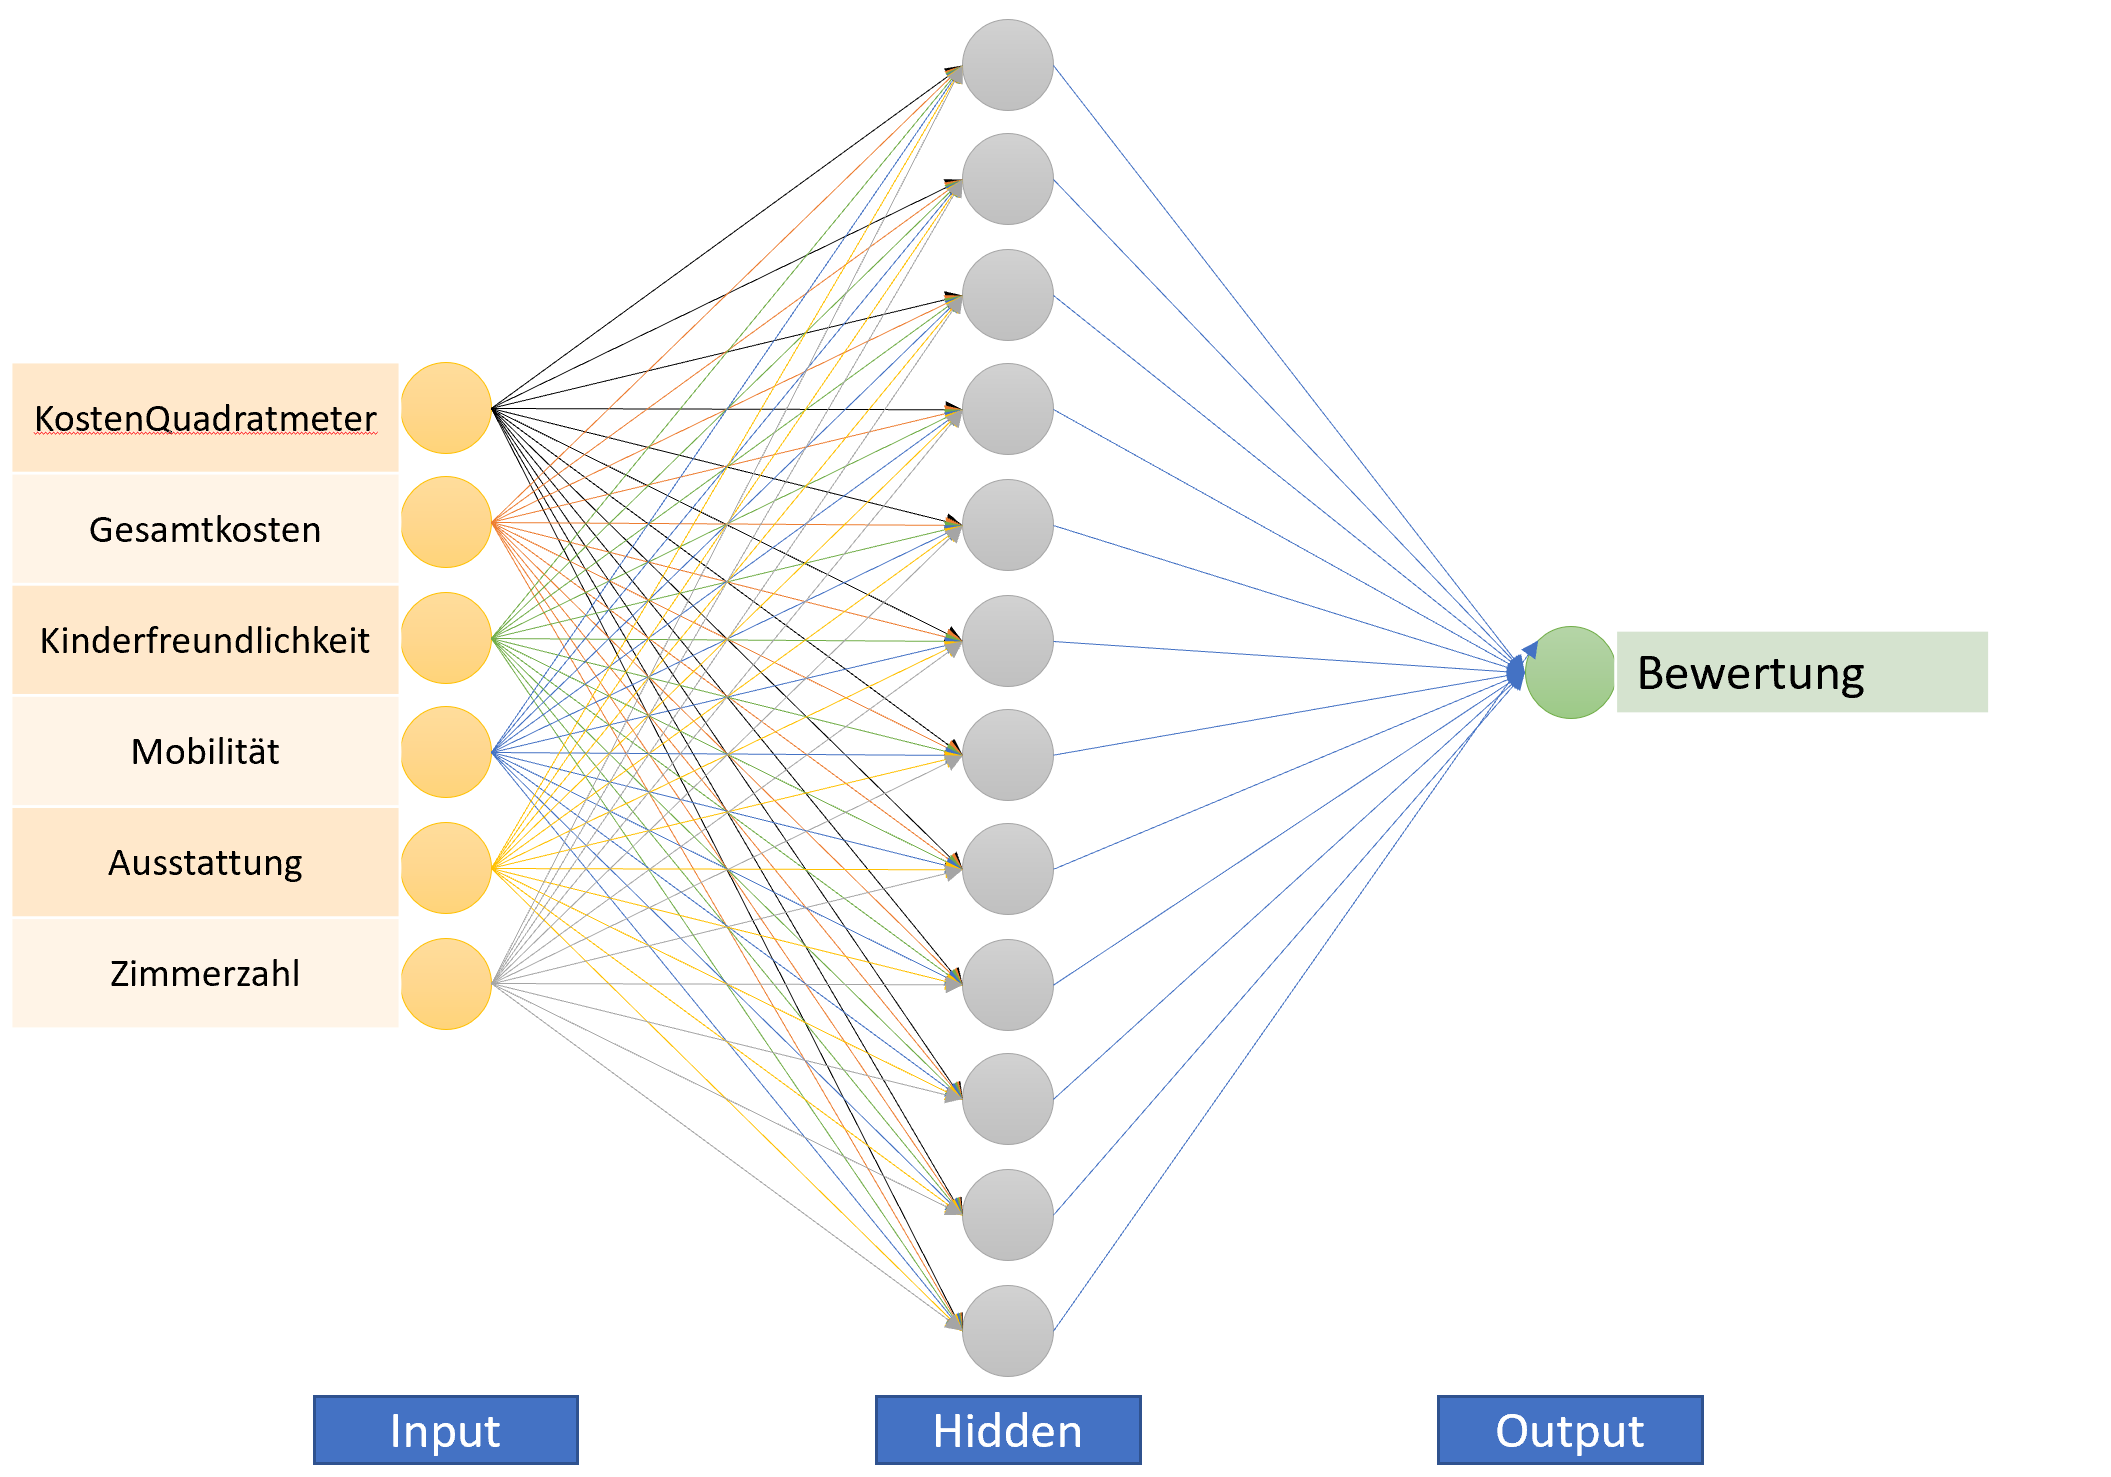
\includegraphics[width=15cm]{NNStruktur.PNG}
        \label{img:nnStruktur}
        \caption{Struktur des Neuronalen Netzes}
\end{figure}

\begin{itemize}
    \item Feed-Forward Netz
\end{itemize}

\subsection{Lernregel}
Die Lernregel sorgt für die Anpassung der Gewichte. 

\subsection{Transferfunktion}
Die Transferfunktion wandelt die normierten Eingabewerte in die Ausgabe der einzelnen Neuronen um.

\begin{equation}
    T_s(x) = \frac{1}{1+e^(\frac{x-S}{k})}
\end{equation}

\subsection{Arbeitsweise/Ablauf}

\begin{enumerate}
    \item Initialisierung
    \item Berechnung der Aktivierung \textit{Hidden-Layer}
    \item Berechnung Ausgabe der \textit{Hidden-Layer} mithilfe der Transferfunktion
    \item Berechnung Aktivierung \textit{Output-Layer}
    \item Berechnung der Ausgabe durch die Transferfunktion.
\end{enumerate}

\subsection{Berechnung der Fehler}

\subsection{Bibliothek Tensorflow zur Implementierung}
Tensorflow ist eine Python-Bibliothek für verschiedene Anwendungen im Bereich Deep Learning. 
Der Name spiegelt das Grundkonzept dieser Bibliothek wieder. 
\textit{Tensor} bezeichnet den Datensatz der in das Deep Learning System 
eingegeben und verarbeitet wird. \textit{Flow} bezeichnet den Ablauf, 
der Verarbeitung des Datensatzes. \\
Beim Erstellen eines Systems mit Tensorflow werden zwei Phasen 
unterschieden. 
Die Bibliothek bietet neben dem generellen Konzept für Maschine Learning Anwendungen 
viele weiter mathematische Funktionen. 
\cite{tf:2018}

\subsection{Konzept zur Implementierung mit Tensorflow}
\subsubsection{Lernrate und Lernschritt}
Tensorflow bietet verschiedene Verfahren für konstante und variable Lernraten. 
Als Start für eine konstante Lernrate bietet sich der Wert 0,5 an. Jedoch bietet 
die Implementierung einer variablen Lernrate einige Vorteile. Die Lernrate kann während 
eines Lernschritts erhöht oder verringert werden. Dies steigert die Effizienz des Algorithmus. 
\autoref{lst:nnVariableLernRate} zeigt die Implementierung mithilfe von Tensorflow. 
Die Lernrate wird hier alle 100000 Schritt mit der Basis 0,96 erhöht. 

\lstinputlisting[
    float,
    floatplacement=H,
    caption=Implementierung einer variablen Lernrate,
    label=lst:nnVariableLernRate,
    language=Python
]{nnVariableLernRate.py}

Durch die Minimierung des \textit{global step} wird die Lernrate erhöht. 
Die Definition des Lernschrittes ist in \autoref{lst:nnLernSchritt} dargestellt.
Während jedem Lernschritt werden die Gewichte des Netzes optimiert.
Dies wird mit einer Kostenfunktion ermittelt. 
Die \textit{softmax cross entropy with logits} normiert zunächst die Werte auf Werte zwischen 0 und 1 und berechnet im 
Anschluss den Fehler zwischen berechnetem Wert und gefordertem Wert.

\lstinputlisting[
    float,
    floatplacement=H,
    caption=Implementierung des Lernschrittes,
    label=lst:nnLernSchritt,
    language=Python
]{nnLernschritt.py}

\subsubsection{Initiale Gewichte}
Die initialen Gewichte für das Netz werden zufällig gesetzt. Diese werden in der Lernphase 
mit hilfe einer Kostenfunktion angepasst.

\subsubsection{Aufbau des Perceptrons}
Die Anzahl der Schichten wird anhand der Anzahl der Eingabewerte ermittelt. 
Durch die Reduzierung der Eingabeattribute in der Vorverarbeitung sind nun lediglich 6 Neuronen in 
der Eingabe-Schicht notwendig. Eine Handregel besagt die Anzahl der versteckten Schichten sollte mit
$Anzahl Hidden Layer = Eingabeneuronen/2$ berechnet werden. Demnach sind 3 versteckte Schichten notwendig. 
Die Ausgabe des Netzes soll das Attribut \textit{Bewertung} sein. Demnach enthält die 
Ausgabe-Schicht lediglich ein Neuron.\\
\autoref{lst:nnModel} zeigt die Implementierung eines solchen Perceptrons. Die \textit{matmul} Funktion 
berechnet hierbei eine Matrixmultiplikation zwischen vorhergehender Schicht, Gewichten dieser Schicht und der Neigung dieser Schicht.
\lstinputlisting[
    float,
    floatplacement=H,
    caption=Implementierung des Perceptrons,
    label=lst:nnModel,
    language=Python 
]{nnModel.py}

\subsection{Zusammenfassung}
Die Tensorflow-lib eignet sich sehr gut für die Entwicklung von Deep Learning Systemen. \\
Sie bietet sehr viele Funktionalitäten, die allerdings bei kleinen Beispielen, sehr kompliziert 
werden können.\\
Das Problem der Wohnungsbörse ist ein Problem, dass durchaus mit einem neuronalen Netz gelöst werden kann. 


